\chapter{$K_S^0$ reconstruction study}

The final states of $B^0 \to K_S^0  K_S^0  K_S^0 $ only depends on the decay of $K_S^0$. The main decay channels of $K_S^0$ is to either $\pi^+ \pi^-$ at branching fraction of about 0.692, or to $\pi^0 \pi^0$ at branching fraction of 0.307, referenced from PDG\cite{pdg}.
 The characteristics of these two decays are much different in terms of the response from the Belle II detector. The charged decay that yields  $\pi^+ \pi^-$ leaves two tracks originating from VXD or CDC volumes with opposite charges. On the other hand, the $\pi^0$ main decay channel is $\pi^0 \to \gamma \gamma$ which typically results in the photon clusters on the ECL. There are mainly two reasons for not selecting $\pi^0$ as final states.
 First, $\pi^0 \to \gamma \gamma$ can yield a large fraction of fake $K_S^0$. The reconstruction of two photons using ECL clusters provides no constrain on $K_S^0$ vertex so it's almost impossible to suppress the combinatorial background using vertexing quality in this case. The photons could be originating from many other resources, such as beam background and charged track radiation. Besides, the main viable selection is the mass of $K_S^0$ which is typically distributed around its nominal mass with a few hundred of keV. However, using the mass window of $K_S^0$ could not effectively reject the noticeable fraction of fake $K_S^0$, especially when using photons. Second, $B^0$ that decays to one or more $K_S^0$ reconstructed from neutral pions have poorly reconstructed vertices. Even with $B^0 \to K_S^0  K_S^0  K_S^0 $ which only uses $K_S^0$ from charged pions in the final states, there is no direct charged tracks from IP, which leads to the worse resolution of vertex position compared to the channel like a $B^0 \to J/\psi K_S^0$, which has two direct charged tracks of $e^+e^-$ or $\mu^+ \mu^-$ from $J/\psi$. If one (or more) of $K^0_S$ has the poor vertexing quality from its decay products, it can further reduce the precision of vertex positions of $B^0$, which eventually leads to a large uncertainties in defining the decay time of signal $B^0$ and the decay time difference as the key observables of TDCPV measurement. Therefore, only $K_S^0$ reconstructed using charged pions is considered to reconstructed $B^0$ in this analysis.
 
 \section{Cut-based $K_S^0$ Reconstruction}
 
 The $K_S^0$ has average life time at $(8.954 \pm 0.004) \times 10 ^{-11} \:\text{s}$ in PDG. Therefore, the flight length of $K_S^0$ is comparable with the scale of VXD size. In the Belle II energy scale, the flight length of $K_S^0$ is in a range from a few $\mu$m away from $B$ vertex to more than 13.5 cm that is further than the outmost layer of SVD ladders, see Figure \ref{fig:ks_flight}.

 % check this plot for how to normalize
 \begin{figure}[htpb]
 	\centering 
 	\begin{minipage}[t]{0.45\linewidth}
 	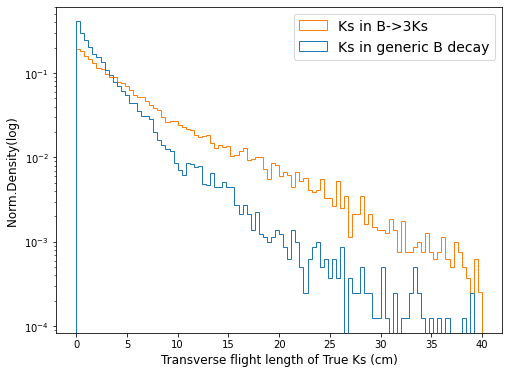
\includegraphics[width=0.9\linewidth]{ks_flight_XY}
 	\end{minipage}
	\begin{minipage}[t]{0.45\linewidth}
		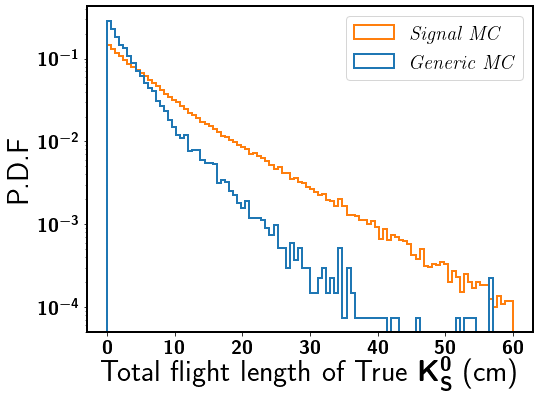
\includegraphics[width=0.9\linewidth]{ks_flight_All}
	\end{minipage}
 	\caption{The left is the transverse flight length distribution and the right is the total flight length distribution from true $K_S^0$.  The blue is from generic MC and  the orange is from signal MC. Both plots are normalized.}
 	\label{fig:ks_flight}
 \end{figure}
 
 Due to the different topology of $B^0$ decay, the average momentum of $K_S^0$ in generic MC is different from the ones from the signal MC. In general, the cut-based reconstruction for $K_S^0$ is first performed by the selection of invariant mass from its decay products. After the selection on invariant mass is applied, a vertex fit for each $K_S^0$ using two reconstructed charged pions is done without IP constraint. This reconstruction is mainly achieved by using standard BASF2 particle list, in which two $K_S^0$ collections are first reconstructed and then merged. We first take all the V0 objects from BASF2 which use 2 online reconstructed charged tracks with opposite charges and a converged fitted vertex. In this step, charged tracks with mass hypothesis of $\pi^{\pm}$ is used, which the tracks and PID of charged pions are pre-selected by the criteria in Table \ref{tab:kspipi_select}. The $K_S^0$ candidates with invariant mass $M$ between $0.45 < M < 0.55$ GeV are selected. In addition to these $K_S^0$ from V0 objects, another $K_S^0$ collection from offline reconstruction is also formed. The V0 based $K_S^0$ and offline reconstructed $K_S^0$ are merged and the vertex fit is performed using ``TreeFit"\cite{krohn2020global}. The duplication of $K_S^0$ between two $K_S^0$ collections are possible. Therefore, the objects' index of two charged pions' tracks in BASF2 are compared, from which the identical combinations are removed to avoid duplication. The $B^0$ reconstruction efficiency is highly sensitive to the efficiency of charged pions because the final state particles are three identical $K_S^0$ decaying to six charged pions. That's why a very loose selection on $\pi^{\pm}$ is applied. The selected $K_S^0$ collection using cut-based method contains many fake candidates from signal MC as shown in Figure \ref{fig:ksM_sigmc}.
\begin{table}[htbp]
	\centering
	\large
	\caption{Pre-selection criteria of $\pi^+ \pi^-$ for $K_S^0$ reconstruction.}
	\label{tab:kspipi_select}
	\begin{tabular}{c c c c }
		\toprule
		Selection & $\theta$ & CDC Hits Number & PID  \\
		\hline
		Criteria  & CDC acceptance &  $>20$ & pionID $> 0.1$\\
		\bottomrule
	\end{tabular}
\end{table}

% check y-axis and how many ks here.
\begin{figure}[ht]
	\centering 
	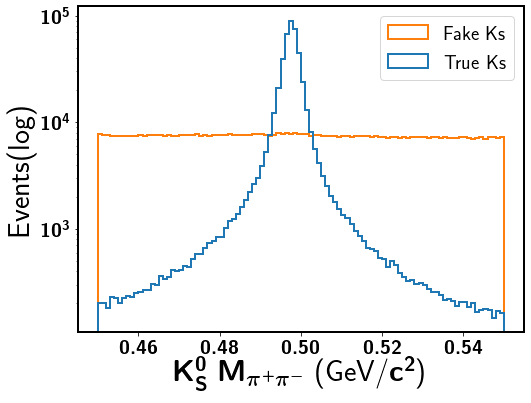
\includegraphics[width=0.6\linewidth]{Ks_M}
	\caption{``M" of $K_S^0$ from cut-based selection in signal MC. The blue line is the true $K_S^0$ and the orange is the fake $K_S^0$. 200000 candidates are used in total. }
	\label{fig:ksM_sigmc}
\end{figure}
\begin{comment}
The $K_S^0$ candidates from ``stdKshort:merged" is the default way to obtain $K_S^0$ in the current BASF2, 
however, the limitation of this cut-based $K_S^0$ reconstruction is the pollution from fake $K_S^0$. Using these $K_S^0$ candidates to reconstruct $B^0 \to K_S^0  K_S^0  K_S^0$, as long as one of three $K_S^0$ is fake, the reconstructed $B^0$ is fake, too. 
\end{comment}

 The reconstruction quality of $K_S^0$ also depends on the flight distance. $K_S^0$ that decay in the inner region of VXD yields more hits on the SVD layers from its charged daughters, which is critical in performing a proper tracking. Belle II tracking efficiency gets poor due to higher beam background when performing track finding for tracks without inner detector hits such as SVD. For certain fraction of $K_S^0$ decaying outside of layer 5 of SVD, it's much likely that there is no SVD hits assigned to their daughters' tracks. This is due to the feature of SVD track finding, where a track candidate needs either at least 3 SVD hits to form a good SVD track, or 2 hits to form a hit double-lets to be used as a complete track. Single hit on layer 5 or layer 6 is filtered out to suppress the large fraction of beam background induced by random single hits. This effect is shown in Figure \ref{fig:ks-r-svdxx}. $K_S^0$ are categorized based on how many SVD hits their daughters have, in which \textit{SVD10} and \textit{SVD01} stands for $K_S^0$ that only $\pi^+$ and $\pi^-$ has non-zero SVD hits number, \textit{SVD11} and \textit{SVD00} stands for $K_S^0$ that both or neither charged pions have SVD hit non-zero SVD hits number. This is related to the track quality of $K_S^0$ where \textit{SVD11} $K_S^0$ has the best quality and \textit{SVD00} has the worst. Thus, the efficiency and purity of $K_S^0$ with long flight length is reduced. It's clear that \textit{SVD00} $K_S^0$ show up at about 11 cm where SVD layer 5 is placed. Most of \textit{SVD10}(\textit{SVD01}) $K_S^0$ start to show up at the similar range. The geometric structure of PXD and SVD is shown in Figure \ref{fig:svdgeo} and the fraction for each types of $K_S^0$ in $B^0 \to K_S^0  K_S^0  K_S^0$ is listed in Table \ref{tab:svdxx}.
\begin{figure}[htpb]
	\centering
	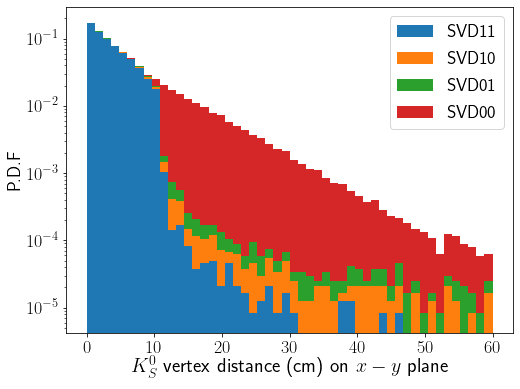
\includegraphics[width=0.7\linewidth]{ks-r-svdxx}
	\caption{$K_S^0$ transverse flight length based on SVD hits of pions. \textit{SVD11}: both pions have SVD hits, \textit{SVD10}(\textit{SVD01}), positive(negative) pions have SVD hits, and \textit{SVD00}: no SVD hits from pions. The result is from signal MC of $B^0 \to K_S^0  K_S^0  K_S^0$.}
	\label{fig:ks-r-svdxx}
\end{figure}

\begin{table}[H]
	\centering
	\begin{tabular}{|c|c|c|c|c|}
		\hline
		$K_S^0$ type & SVD11 & SVD00 & SVD10 & SVD01\\
		\hline
		\% in Belle II & 52\% & 39\% & 5\% & 5\%\\
		\hline
	\end{tabular}
	\caption{The fraction of each category of $K_S^0$ based on pions SVD hits in $B^0 \to K_S^0  K_S^0  K_S^0$ signal MC.}
	\label{tab:svdxx}
\end{table}
\begin{comment}
\begin{figure}[htpb]
\centering
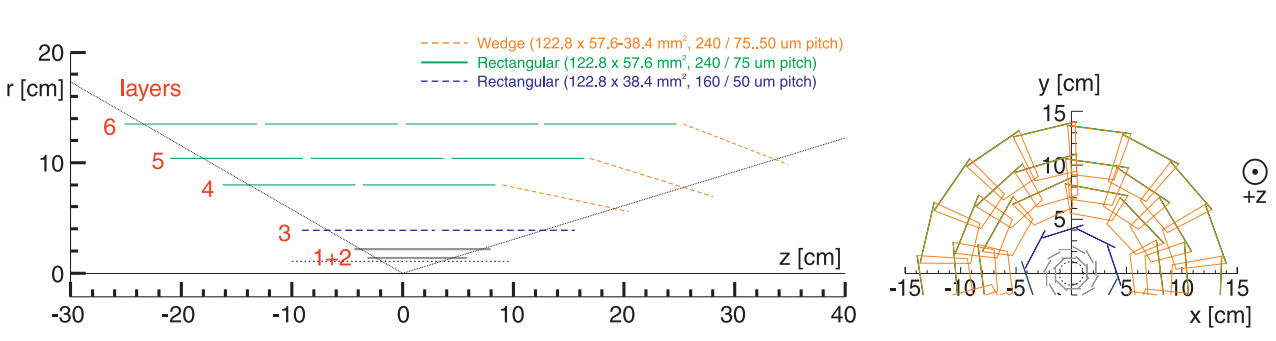
\includegraphics[height=4cm]{VXDGEO.png}
\caption{Geometric structure of PXD and SVD in Belle II\cite{Abe:2010gxa}. SVD Layer 5 is at $r = 11$ cm and $K_S^0$ that decay outside are very likely to lose SVD hits information.}
\label{fig:vxdgeo}
\end{figure}
\end{comment}


Fake $K_S^0$ candidates costs a large extra processing time and the number of combinatorial backgrounds in $B^0 \to K_S^0  K_S^0  K_S^0$ becomes high, which largely reduces the signal significance and introduce bias to the $\it{CP}$ parameters measurement. Thus, a multi-variate analysis (MVA) based $K_S^0$ classification package, \textit{KsFinder}, is developed to further reject the fake $K_S^0$ from cut-based selected candidates.


% 2021.02.03 ends
\section{MVA-based $K_S^0$ selection}

\subsection{Belle II $K_S^0$ classification}
As mentioned in the last section, in order to improve the reconstruction performance of $K_S^0$ from cut-based selection, a MVA-based package called ``KsFinder" has been developed. The reconstruction of $K_S^0$ can be treated as a typical classification problem. The input is a set of variables that describes the characteristics of $K_S^0 \to \pi^+ \pi^-$ decay. The training  target is the true or fake flag from the MC truth-matching variable called ``isSignal" where isSignal = 1 (0) stands for being a true (fake) $K_S^0$. It aims to improve the limitations in the Belle $K_S^0$ MVA classification tool. 
 
 In Belle, the $K_S^0$ reconstruction was first done by using cut-based method to select primary candidates, then a MVA-based classifier was implemented by assigning two likelihood indicators to each $K_S^0$ candidates. The package used by Belle is called \textit{nisKsFinder}\cite{b2book} which outputs the two likelihood variables based on NeuroBayes algorithm\cite{feindt2006neurobayes}. The Belle tool defines the goodness of $K_S^0$, called \textit{nb\_nolam} and \textit{nb\_vlike}, respectively. As their names suggest, \textit{nb\_nolam} is the likelihood of not being a $\Lambda$ particle and \textit{nb\_vlike} is the likelihood of being a V0-like particle. A good $K_S^0$ candidate from \textit{nisKsFinder} is the one with a low likelihood of being $\Lambda$ particle and a high likelihood of being a V0-like particle, assuming the major backgrounds for $K_S^0$ is the mis-identified $\Lambda$ among V0-like particles. By putting cuts on these two variables, a purification of $K_S^0$ can be made, see Figure \ref{b1niskf}. It can effectively reduce fake $K_S^0$ from cut-based selected candidates, however, there are a few disadvantages about this method. First, NeuroBayes is a commercial product that was developed over 10 years ago. The official support and update is stopped nowadays, so it's not an ideal method for an experiment like Belle II that has a quite long prospective in operation. Second, the classification is based on a joint cut on two variables, which might make the cut values hard to choose, for example, two different cuts might have very close purity. Last but not least, the classification of $K_S^0$ is not the directly targeted output of the neuro-network. Instead, it classifies the V0-like particle and ``$\Lambda$". Besides, the computation speed of NeuroBayes is not optimized.

\begin{figure}[htpb]
	\centering 
	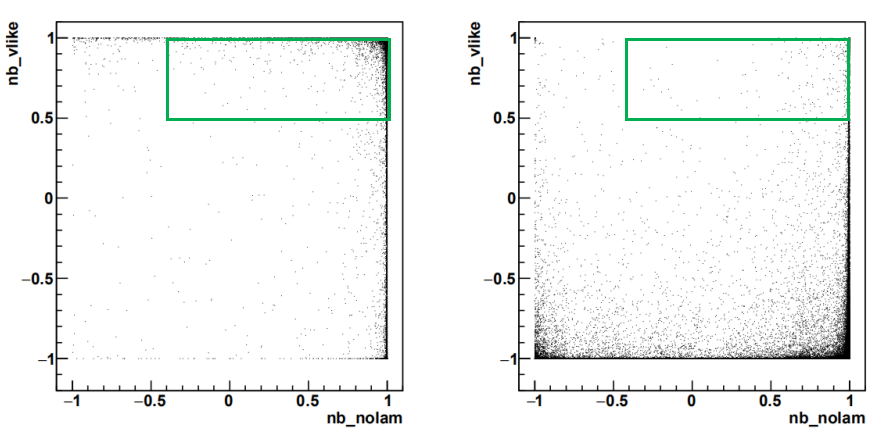
\includegraphics[width=0.7\linewidth]{nisksfinder}
	\caption{The distribution of two variables outputs: \textit{nb\_nolam} and \textit{nb\_vlike} for $K_S^0$ candidates from Belle signal MC. The left is from true $K_S^0$ and the right is from the fake $K_S^0$. In Belle, the standard cuts for $K_S^0$ is \textit{nb\_vlike} $> 0.5$ and \textit{nb\_nolam} $> -0.4$\cite{kang2020measurement}.}
	\label{b1niskf}
\end{figure}


Such a dedicated $K_S^0$ classification tool is not implemented yet in BASF2 framework until 2019. Considered the limitation of NeuroBayes, the development of $K_S^0$ classifier demands another algorithm and structure. The \textit{Boosted Decision Trees} (BDT) is widely employed for multivariate classification and regression tasks in high energy physics field. Particularly, a speed-optimized and cache-friendly
implementation of such a method called FastBDT (FBDT) is popularly used\cite{keck2016fastbdt}. Compared to other popular classification algorithms such as TMVA\cite{therhaag2012tmva}, scikit-learn\cite{pedregosa2011scikit} and XGBoost\cite{chen2016xgboost}, FastBDT method is proven to be one order of magnitude faster during the training and applying phases\cite{keck2016fastbdt}. 
By using FastBDT algorithm, KsFinder in Belle II is expected to give a single output which directly presents the goodness of a candidate of being a true $K_S^0$. Since the FastBDT algorithm depends on the variables that are different in signal and backgrounds, a set of training variables are selected based on $K_S^0$ decay topology.  The $K_S^0$ variables used in the training of KsFinder might be differently distributed in different decay channels, therefore a KsFinder trained using MC sample from one channel may not be able to perform a good classification on the other. Thus, KsFinder is designed as a general package that provides a mode-dependent $K_S^0$ classification which mainly consists of four components: \textit{KsFinderSampler}, \textit{KsFinderTeacher}, \textit{KsFinderApplier} and \textit{KsFinderTest}. KsFinderSampler is a function that automatically generates training and/or testing sample from mDST files where the cut-based reconstruction is used as section 3.1. KsFinderTeacher is responsible for extracting variables to perform training of the FastBDT model and generate a weight file containing all the nodes information in ROOT format, which also provides a function to communicate with BASF2 CDB so that users can share or download others' weight file in their own analysis. KsFinderApplier can apply the weight file generated by KsFinderTeacher (or downloaded from BASF2 CDB) to the independent data sample and assign each $K_S^0$ candidate a goodness index used as a single cut value in the further analysis. KsFinderTest is the evaluation function that can use a test sample to check for over-training, efficiency, purity.  By providing MC sample(s) from a certain decay mode(s), users can easily generate their own weight file(s) of $K_S^0$ classification that suits different decay modes despite $K_S^0$ variables distribution may be varied. Such a design largely improves the flexibility of KsFinder compared to Belle MVA tool which indirectly classify $K_S^0$ with two outputs. 

\begin{comment}
\subsection{FastBDT algorithm}
As the basic component of BDT, a general DT (decision tree) performs classification using a number of consecutive cuts at each tree nodes, where tree nodes are distributed on the layers of a tree. The maximum number of the layers is called ``depth of tree" and it's a hyper-parameter of a DT. Each data point contains labels (variables) called ``features" in DT. There are generally two phases in using DT for classification. One is ``training" (or ``fitting") phase that determines the best cut at each nodes. The other is called ``applying" phase that uses a trained DT to classifier a new data set. In training phase, training data points are fed to a DT and separated based on their features. At each node with a cut value, a cumulative probability histogram (CPH) can be defined by counting the signal and background data points. The histograms are used to determine the separation gain for a cut value at each position in these histograms. The feature and cut value (or
equivalently bin) with the highest separation power are used as the cut for the node. Hence, each cut value locally maximizes the separation gain between signal and background on the given
training sample. Eventually, on the last layer (called terminal layer), the signal fraction of all training data points in the same terminal node is used for the signal probability for a testing data point which ends up in the same terminal nodes, shown as Figure \ref{fig:DT}. In applying phase, a new data set, such as a test sample, is fed to the trained DT with fixed cut values at each nodes, to evaluate the performance of a DT or use it to separate the signal and background.

\begin{figure}[htpb]
\centering 
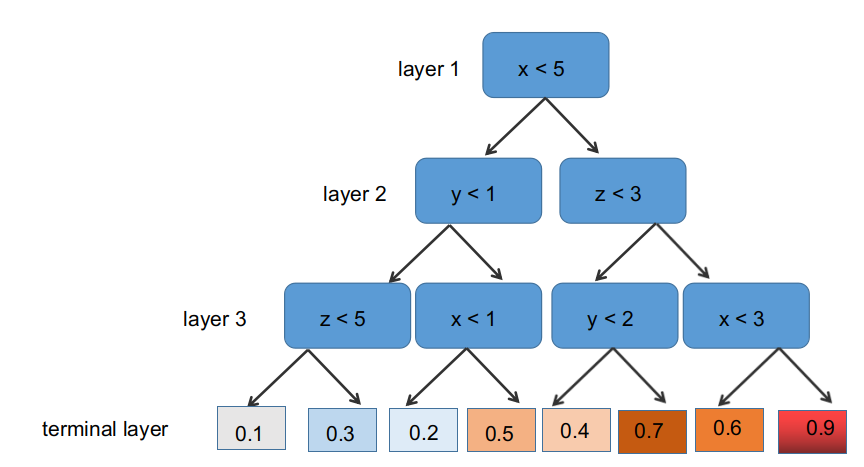
\includegraphics[width=0.7\linewidth]{DT}
\caption{Basic structure of a DT with depth = 3 and labels (features) of x,y,z. The terminal layer contains training data points and are separated by cuts on layer 1 to 3. The number (color demonstrated) is the signal fraction of training data points in each terminal node, which is used for testing data points signal probability.}
\label{fig:DT}
\end{figure}

The mathematical idea behind this method is to treat the data points as a data set defined on a multi-dimension hyper-space. As long as the signal/background data points show certain concentration in a sub-region of the hyper-space, it's possible to locally increase the signal fraction by consecutively cutting on the edge where signal and background are separated. The cut on labels at each node is the edge of the sub-region. A very deep DT (too many layers) means the edges of the sub-region of the hyper-space is cut too finely so that even small statistical fluctuation could be separated. Therefore, training data points in the sub-region can give a over-trained signal fraction that is unrealistically high. As a result, the classifier performs poorly on new data points since the fluctuation is randomly occurred in new data set. There are pruning algorithms which automatically remove cuts prone to over-training
from a DT, details can be found here \cite{olshen1984classification}.

Avoiding the over-training of a DT limits the depth of a tree strongly. For a problem of $K_S^0$ classification, the number of observables (features) is much more than the usual tree depth (a few layers). A single DT can only roughly separate the signal and background and thus, it's called a weak-learner. To improve the separation power, a sequence of many shallow DTs is formed during the training phase. For all the DTs, a negative binomial log-likelihood loss-function is minimized in the training phase. By using the results from many DTs (many weak learners), a well-regularized classifier with large separation power is constructed. The number of trees $N$ is called ``boosting steps", which is also the hyper-parameters for the training model. Such improved model is called ``Boosted Decision Trees" (BDT). There are a few different strategies to further optimize the performance of BDT such as ``Gradient Boost Decision Trees" (GBDT) and ``Stochastic Gradient Boost Decision Trees" (SGBDT) which use different methods to define the model output or increase the training speed, details are discussed here\cite{friedman2002stochastic}.


The FastBDT (FBDT) implements a optimized algorithm from a derived SGBDT method \cite{friedman2001greedy} and gain an order of magnitude faster execution time. FBDT reduces CPU time on CPH for tree nodes by using binned values for comparison to avoid  floating-point data calculation. It uses ``struct of arrays" that leads to a faster pre-cached CPU memory access pattern. The comprehensive comparison in terms of speed in fitting and applying phases between FastBDT and other popular methods such as XGBT, TMVA and scikit-learn is described in here\cite{keck2016fastbdt}. 

\begin{comment}
\begin{figure}[htpb]
\centering
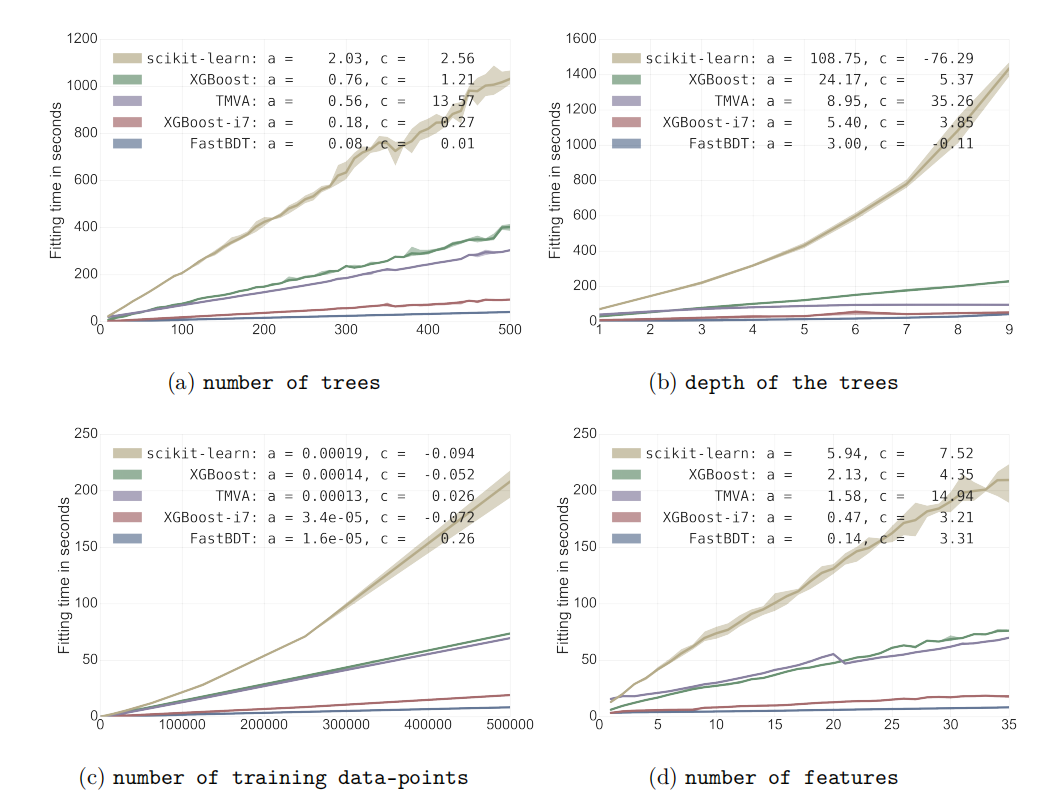
\includegraphics[height=12cm]{speedFBDT}
\caption{Runtime in fitting phase with different hyper-parameters comparison among FastBDT and XGBT,TMVA,scikit-learn.\cite{keck2016fastbdt}}
\end{figure}
\end{comment}

% 2021.02.04 ends


\subsection{Decay Topology of $K_S^0 \to \pi^+ \pi^-$}
As introduced in section 3.2.1, the first step for developing $K_S^0$ MVA classification is to determine the input variables for FastBDT algorithm that can represent the decay features of $K_S^0$ against possible backgrounds.
The remaining background of  $K_S^0 \to \pi^+ \pi^-$ after the cut-based reconstruction comes from different sources, mainly including the false combination of tracks (including $\pi^{\pm}$ misidentification), V0-like particle misidentification and self-looped tracks.
For instance, a $D^0/D^*$ from a $B$ decaying to $K\pi$ with $K$ misidentified as $\pi$, could give a false combination of tracks. On the other hand, it's also possible that both of two tracks are correctly identified as $\pi^{\pm}$ but they are not from the same mother particle, or the mother is not a $K_S^0$ particle due to the missing of other daughters, such as $D^+ \to K_S^0 (  \to \pi^+ \pi^-) \pi^+$. The decay shape resembled the above cases are illustrated in Figure \ref{fig:fakeks1}. 


\begin{figure}[htpb]
	\begin{minipage}[t]{0.5\linewidth} % 如果一行放2个图,用0.5,如果3个图,用0.33
		\centering 
		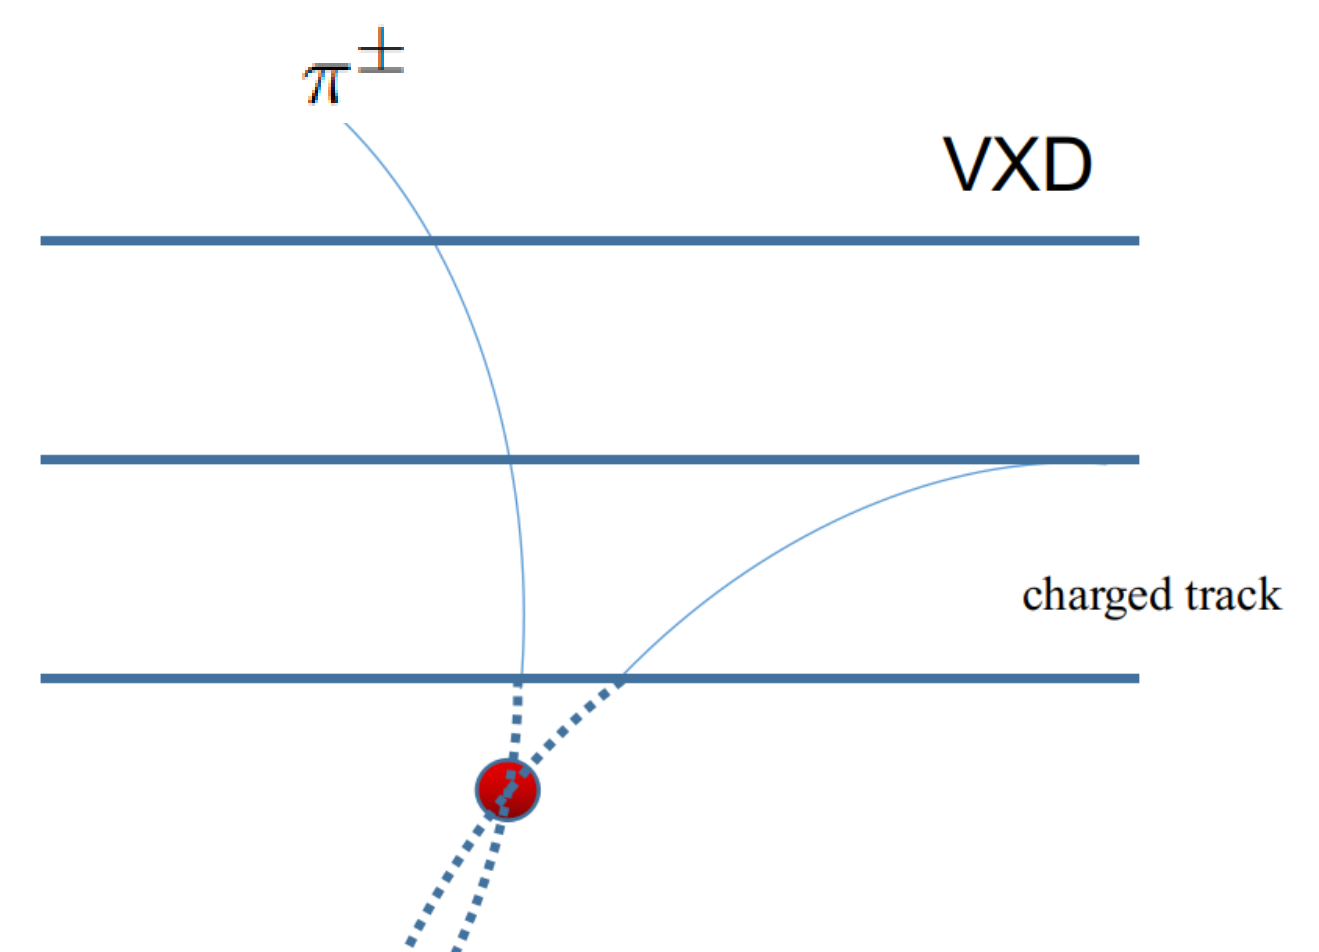
\includegraphics[width=7cm]{fakeks1_1} 
		%\label{fig:side:a} 
	\end{minipage}%
	\begin{minipage}[t]{0.5\linewidth} 
		\centering 
		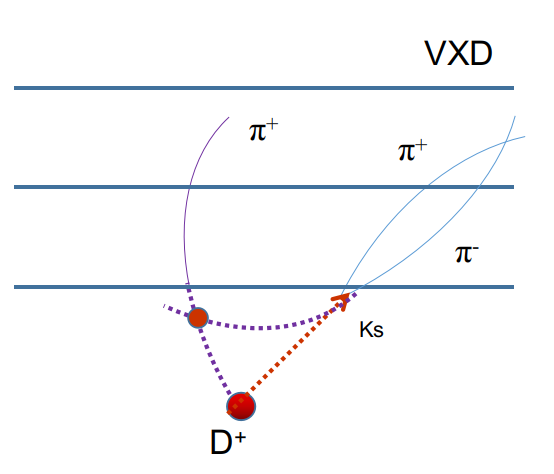
\includegraphics[width=7cm]{fakeks2} 
		%\caption{ } 
		%\label{} 
	\end{minipage}% 
	
	\caption{The left shows the case when a charged track (not $\pi^{\pm}$) combined with a charged pion to form a fake $K_S^0$, the right shows the case when two daughters are correctly reconstructed as pions but not from the correct mother particle, which is falsely taken as a $K_S^0$.}
	\label{fig:fakeks1}
\end{figure}

The V0-like particles mainly refer to $K_S^0$, $\Lambda$ and $\gamma$. $\gamma \to e^+ e^-$ yield is significantly lower than the other two types and the mass different between pion and electron is very large, so the PID values can be used to well-distinguish them. As for the contribution of $\Lambda \to p^+ \pi^-$, it happens when the positive charged tracks (proton track) is wrongly identified as $\pi^+$, see Figure \ref{fig:fakeks2} left. The key observable to distinguish this background is the invariant mass of mother particle, which is 1.115 $\Lambda$ GeV, much larger than the $K_S^0$. The number of left-over $\Lambda$ after the cut-based reconstruction in section 3.1 is small, and can be further reduced by rejecting the candidates whose positive charged daughter has PID($\pi^{\pm}$) smaller than PID($p$).

When a charged pion only carries a minimal of its mother's transverse momentum $p_T$, the curvature of its track may form a self-loop of which radius is comparable with the size of Belle II detector (mainly VXD and CDC). In this case, one charge pion could leave two charged tracks candidates with the opposite charge and similar $p_T$, with a possibility to form a converged vertex to form a fake $K_S^0$, see Figure \ref{fig:fakeks2} right.

\begin{figure}[htbp]
	\begin{minipage}[t]{0.5\linewidth} % 如果一行放2个图,用0.5,如果3个图,用0.33
		\centering 
		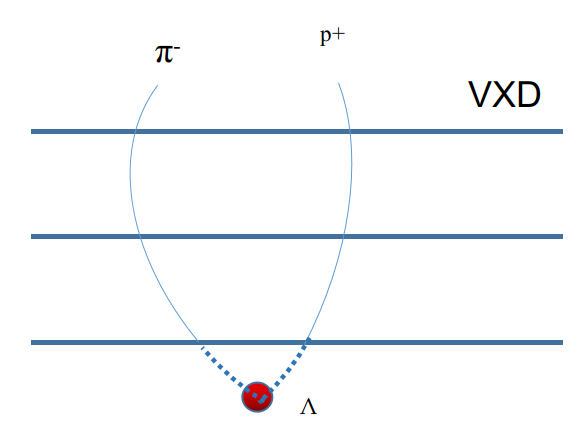
\includegraphics[width=7cm]{fakeks3} 
		\label{fig:side:a} 
	\end{minipage}%
	\begin{minipage}[t]{0.5\linewidth} 
		\centering 
		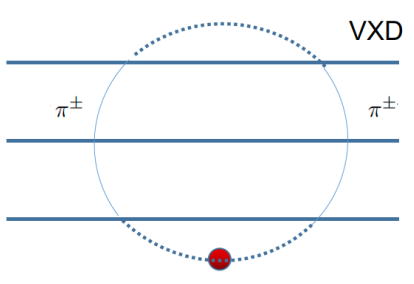
\includegraphics[width=7cm]{fakeks4_4} 
		%\caption{ } 
		\label{fig:side:b} 
	\end{minipage}% 
	
	\caption{The left shows the $\Lambda \to p^+ \pi^-$ decay shape that can be treated as $K_S^0$, the right shows a self-loop formed by a low $p_T$ charged pion reconstructed as two separated tracks with a vertex.}
	\label{fig:fakeks2}
\end{figure}

\subsection{Determination of training observables from $K_S^0$ decay }
Given the characteristics of  $K_S^0 \to \pi^+ \pi^-$ discussed in the previous section, a set of variables as training features of KsFinder can be selected. The set includes variables related to $K_S^0$ kinematics, decay shape parameters, particle identifications and detector hits information. The summarized information of training variables is listed in Table \ref{tab:ks_vars}.

\begin{table}[htbp]
	\centering 
	\small
	\begin{tabular}{|c|c|} 
		\hline
		$K_S^0$ variables &  Meaning \\
		\hline
		{cosVertexMomentum} & cosine between $K_S^0$ vertex and momentum direction (lab)\\
		flight distance & $K_S^0$ flight distance projected on its momentum direction\\
		significanceOfDistance & relative error of flight length from IP\\
		cosHelicityAngleMomentum & cosine between $\pi^{\pm}$ and $K_S^0$ (lab)\\
		ImpactXY & Impact parameters in transverse plane for $K_S^0$\\
		x, y, z, px, py, pz & $K_S^0$ vertex position and momentum\\
		p\_D1(D2) & momentum magnitude for $\pi^+$($\pi^-$)\\
		pionID, muonID & PID values of $\pi^+$\\
		decayAngle\_D1(D2) & angle between $\pi^+$($\pi^-$) and $K_S^0$ ($K_S^0$ CMS)\\
		daughterAngle2body & angle between $\pi^{\pm}$ (lab)\\
		daughtersDeltaZ & Z-direction distance of two tracks helix\\
		nSVDHits\_D1(D2)& SVD detector hits of  $\pi^+$($\pi^-$) \\
		nPXDHits\_D1(D2)& PXD detector hits of  $\pi^+$($\pi^-$) \\
		M, InvM & $K_S^0$ invariant mass before(after) vertex fit\\
		\hline
	\end{tabular}
	\caption{\small Summary of KsFinder input variables, where ``lab" means angles in lab frame and  ``$K_S^0$ CMS" means in $K_S^0$ rest frame. Other variables are calculated in lab frame by default. }
	\label{tab:ks_vars}
\end{table}

\begin{comment}
\begin{itemize}
\item Kinematics
\begin{itemize}
\item invariant mass of $K_S^0$ before and after fitting vertex
\item momentum of $K_S^0$ and $\pi^{\pm}$, vectors and magnitudes. 
\end{itemize}

\item Decay shape parameters
\begin{itemize}
\item cosine angle between $K_S^0$ vertex and momentum in lab frame.
\item helicity angle of two daughters in reference of $K_S^0$ momentum in lab frame.
\item decay angle of two daughters ($\pi^{\pm}$) in the mother's ($K_S^0$) frame. 
\item flight distance projection on $K_S^0$ momentum direction.
\item significance of flight distance, defined by ratio of flight length and its uncertainties.
\item distance of two daughters helix along the Z direction (parallel to beamline).
\item impact parameters on $K_S^0$ vertex
\end{itemize}

\item Particle identifications
\begin{itemize}
\item pion-ID for $K_S^0$ daughters.
\item muon-ID for $K_S^0$ daughters.
\item proton-ID for $K_S^0$ positive charged daughter. 
\end{itemize}

\item Hits information
\begin{itemize}
\item the number of PXD hits for each $K_S^0$ daughter.
\item the number of SVD hits for each $K_S^0$ daughter.
%\item the number of CDC hits for each $K_S^0$ daughter. 
\end{itemize}

\end{itemize}
\end{comment}

The cosine between $K_S^0$ vertex and momentum direction (named ``cosVertexMomentum") is of the most importance because it demonstrates the best separation between a true and a fake $K_S^0$. For instance, if a falsely reconstructed $K_S^0$ is made of two tracks, it's likely that the momentum direction of the fake $K_S^0$ is not aligned with the its vertex direction from IP. So the projection of vertex position of $K_S^0$ on the reconstructed momentum direction could be negative value for fake $K_S^0$. While in case of a true $K_S^0$, such projection is almost always a positive value, shown in Figure \ref{fig:ks_cosvex}. This often happens when the two tracks taken as $\pi^{\pm}$ are accidentally crossed, or due to the misidentified track(s). The abbreviations and importance rank of input variables from KsFinderTest function is shown in Table 
\ref{tab:ks_import}.

\begin{figure}[htbp]
	\centering
	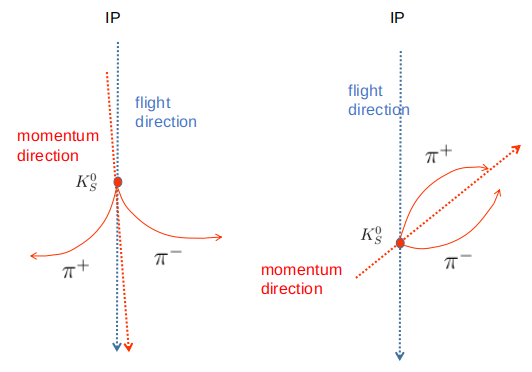
\includegraphics[height=7cm]{ks_cosvex}
	\caption{The left shows a true $K_S^0$ decay shape where the cosine angle of $K_S^0$ vertex position (blue dashed arrow) against reconstructed momentum direction (red dashed arrow) is positive. While the right shows a fake $K_S^0$ decay shape where cosine angle of $K_S^0$ vertex position against reconstructed momentum direction can be negative. }
	\label{fig:ks_cosvex}
\end{figure}
 
As a FastBDT method relies on the distribution of variables to calculate signal and background separation, there are a few points to be checked before feeding the training data to the algorithm or applying the classification. First, the distribution of the observables should be different in true $K_S^0$ and the fake ones, so the FastBDT classifier can effectively separate the true and the fake $K_S^0$ at each node to maximize the separation gain. Second, there will a correlation among the training observables and they should also be different in signal and background. The boosting step will create a sequence of shallow DTs whose structures are not same. Different correlations helps improve the performance of DTs in tuning of structure. For instance, a true $K_S^0$ flights longer due to larger momentum in general, so its daughters' detector hits number becomes fewer. Then these two observables have negative correlations in true $K_S^0$. In case a fake $K_S^0$, the flight length could be a deep outside of VXD  but daughters may have full hits on SVD, without strong correlation, see Figure  \ref{fig:ks_cov} . At last, one should also avoid using many observables with too strong correlations, since in this case, many DTs might have a potentially equivalent structure in the boosting step. Therefore, the separation power of many DTs doesn't gain any improvement and the collection of observables might be redundant. The correlation between variables are shown in Figure \ref{fig:ks_cov}.

\begin{figure}[ht]
\centering
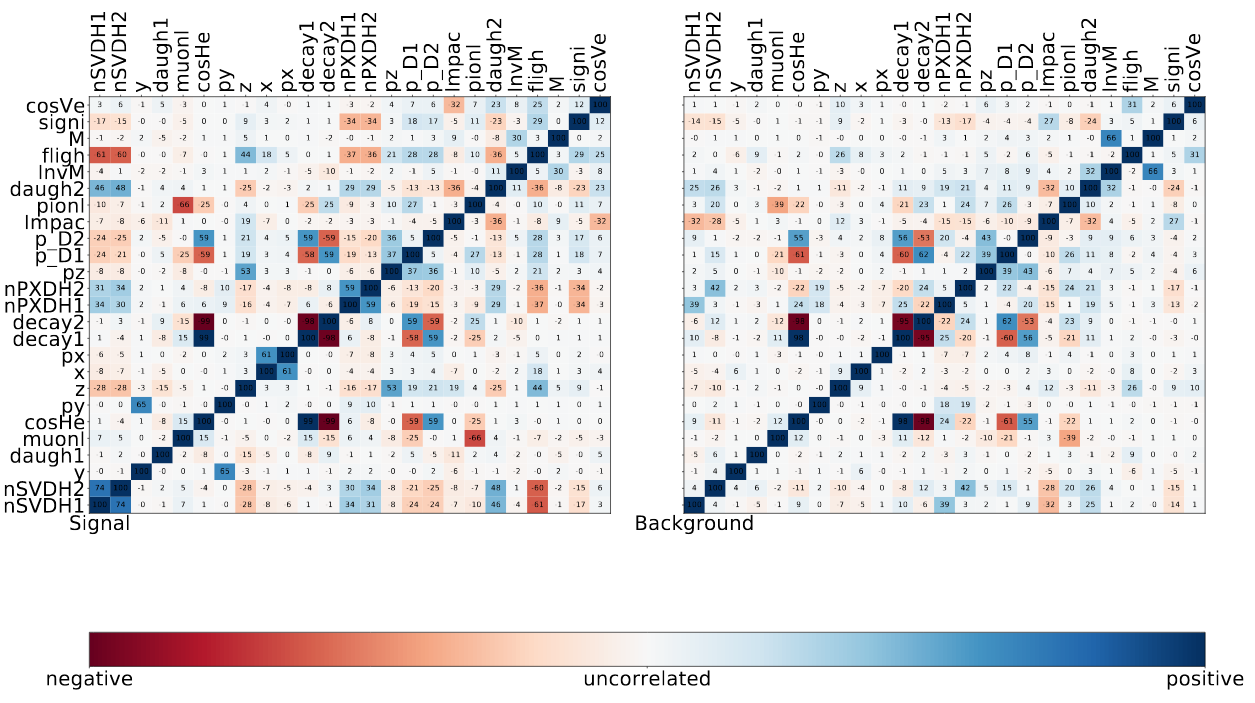
\includegraphics[width=0.8\linewidth]{ks_cov}
\caption{The correlation between input variables for KsFinder. As the given example, flight length has negative correlation with SVD hits in signal while un-correlated in background.}
\label{fig:ks_cov}
\end{figure}

 \begin{table}[htpb]
 	\begin{minipage}[ht]{0.5\linewidth}
 		\centering
 		%\caption{The Abbreviations.}
 		\begin{tabular}{c|c}
 			\hline
 			Observables &  Abbreviations\\
 			\hline
 			nPXDHits\_D1 &  nPXDH1 \\
 			decayAngle\_D1 & decay1 \\
 			nPXDHits\_D2 & nPXDH2\\
 			y & y \\
 			decayAngle\_D2 & decay2\\
 			px & px\\
 			z & z \\
 			cosHelicityAngleMomentum & cosHe\\
 			x & x \\
 			daughtersDeltaZ & daugh1\\
 			nSVDHits\_D1 & nSVDH1\\
 			py & py\\
 			muonID\_pi & muonI\\
 			nSVDHits\_D2 & nSVDH2\\
 			p\_D1 & p\_D1\\
 			p\_D2 & p\_D2\\
 			pz & pz \\
 			flightDistance & fligh\\
 			pionID\_pi & pionI\\
 			InvM & InvM \\
 			daughterAngle2body & daugh2\\
 			ImpactXY & Impac \\
 			significanceOfDistance & signi \\
 			M & M \\
 			cosVertexMomentum & cosVe \\
 			\hline
 		\end{tabular}
 		%\label{fig:side:a} 
 	\end{minipage}
 	\begin{minipage}[ht]{0.5\linewidth}
 		\centering 
 		%\caption{Importance rank }
 		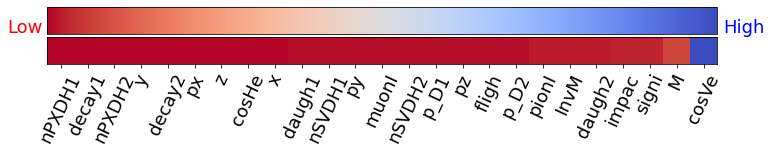
\includegraphics[width=4cm]{rank1}
 		%\label{fig:side:b} 
 	\end{minipage}
 \caption{The abbreviations (left) and importance rank (right) of input variables from KsFinderTest, where the most important variable is ``cosVertexMomentum".}
 \label{tab:ks_import}
 \end{table}




 % 2021.02.05 mid
\subsection{Training, Applying and Testing of KsFinder}
The variables are internally registered inside the KsFinder so it can automatically retrieve their values from a mDST file in BASF2. The first step of using KsFinder is to call KsFinderSampler on a MC sample to generate training and testing data sample. To show the flexibility and stability of KsFinder on different modes, KsFinderSampler extracts MC data points from both signal MC and generic MC (see MC definition in section 2.9), respectively.  KsFinder configures that the depth of each DT is 3 and boosting steps is 200. In both MC samples, the ratio of true and fake $K_S^0$ is set to 1:1 and each component contains 200000 data points. The distribution of input variables in signal MC is shown in Appendix A. 

To train the KsFinder, KsFinderTeacher function is called for the training samples from signal/generic MC and weight files are saved. To apply the classification of $K_S^0$, KsFinderApplier reads in the testing samples of signal/generic MC and calculate output using saved weight files, so that each $K_S^0$ candidate is assigned with a goodness index named \textit{FBDT\_Ks}. It ranges from 0 to 1 where 1 stands for the best goodness. After the applying of KsFinder on the testing samples, KsFinderTest is called to check the performance and over-training of KsFinder on the testing samples, which will be discussed in the next section. 

\subsection{The Performance and Over-fitting check}
To evaluate the performance of KsFinder on both signal and generic MC samples, signal efficiency and background rejection are calculated by cutting on the different values on \textit{FBDT\_Ks}, as defined in Equation \ref{eq:ks_eff} and \ref{eq:ks_rej}.

\begin{eqnarray}
	\text{signal efficency} = \frac{\text{Number of true $K_S^0$ with FBDT\_Ks $>$ cut value}}{\text{Number of all true $K_S^0$ }} \label{eq:ks_eff}\\
	\text{background rejection} = \frac{\text{Number of fake $K_S^0$ with FBDT\_Ks $<$ cut value}}{\text{Number of fake true $K_S^0$ }} \label{eq:ks_rej}
\end{eqnarray}

The ROC (receiver operating characteristics) curve is usually taken as an indicator of the performance where the curve shows the dependence of rejection power with respect to the signal purity. The larger area under a ROC curve means that the better performance is achieved since background rejection drops slower when increasing the cut. The ROC curves and efficiency/background rejections are shown in Figure \ref{fig:3Ks_performance} and \ref{fig:gen_performance}, where the former is for signal MC and the latter is for generic MC.

\begin{figure}[H]
	\begin{minipage}[b]{0.5\linewidth}
		\centering 
		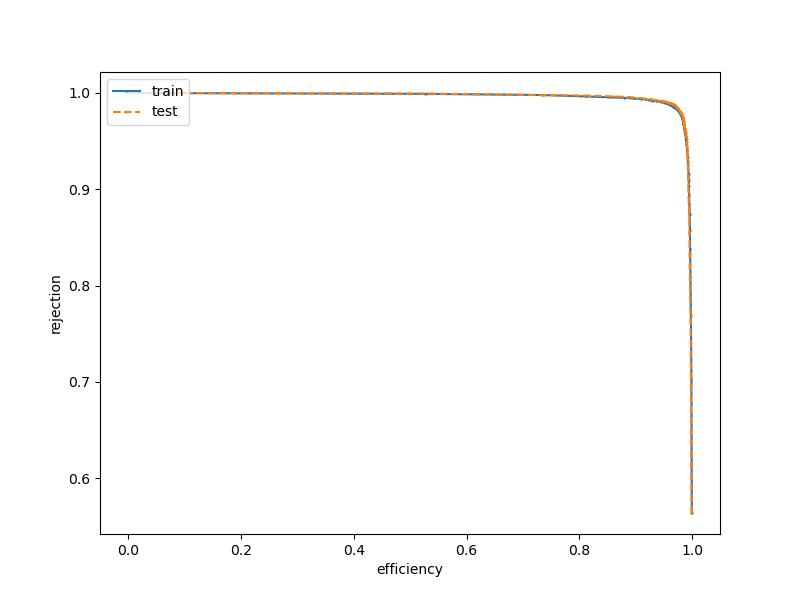
\includegraphics[height=6cm]{ROC_3Ks}
		\label{fig:ROC_3Ks}
	\end{minipage}
	\begin{minipage}[b]{0.5\linewidth}
		\centering 
		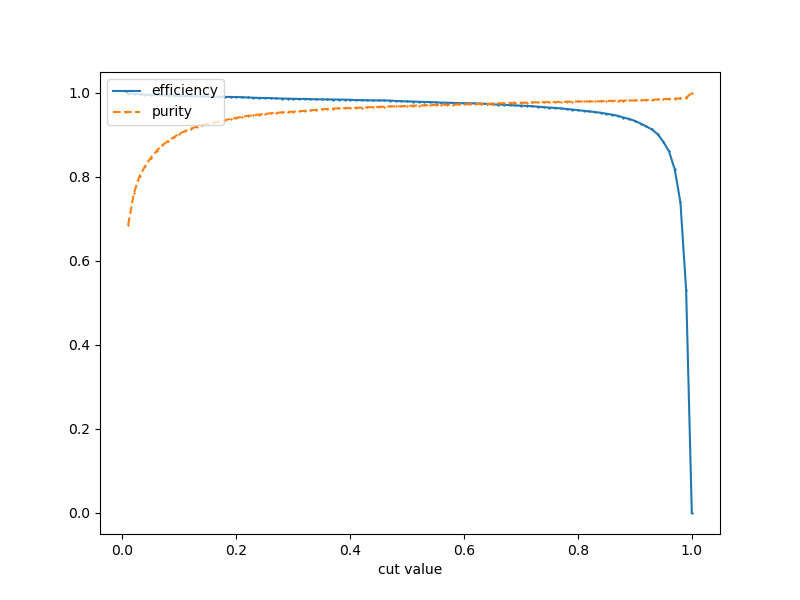
\includegraphics[height=6cm]{eff_3Ks}
		\label{fig:eff_3Ks}
	\end{minipage}
\caption{The left is ROC curve(blue for training and orange for testing) and the right is efficiency and purity (blue for efficiency and orange for purity) depending on cut of KsFinder output. Results are from signal MC sample.}
\label{fig:3Ks_performance}
\end{figure}

\begin{figure}[H]
	\begin{minipage}[b]{0.5\linewidth}
		\centering 
		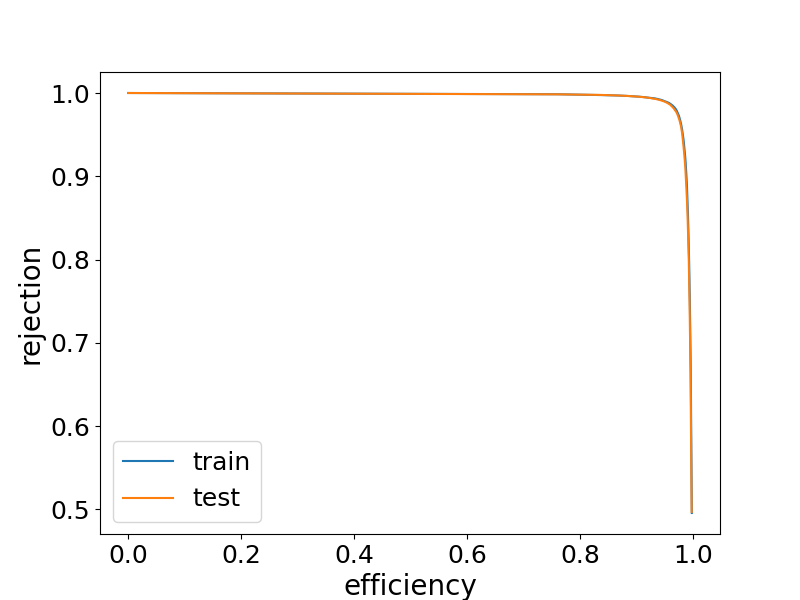
\includegraphics[height=6cm]{ROC_gen}
		%\label{fig:side:a}
	\end{minipage}
	\begin{minipage}[b]{0.5\linewidth}
		\centering 
		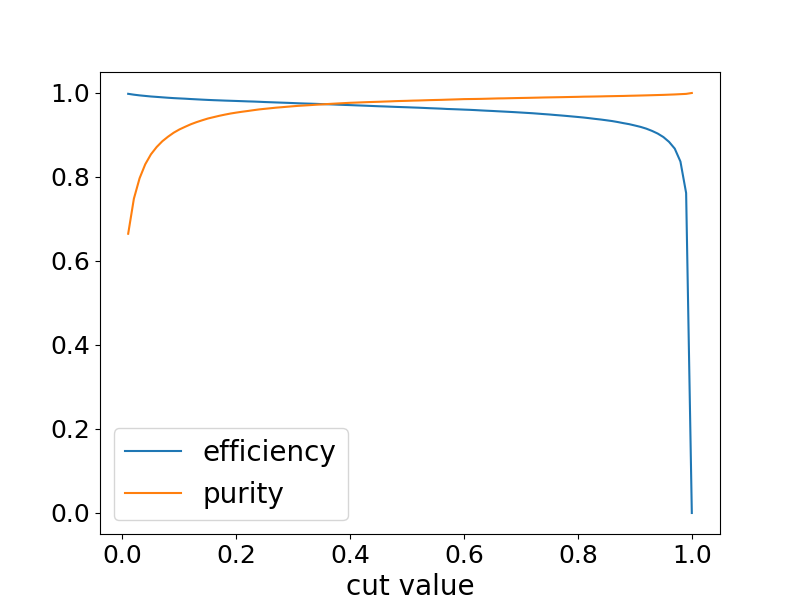
\includegraphics[height=6cm]{eff_gen}
		%\label{fig:side:b}
	\end{minipage}
	\caption{The left is ROC curve (blue for training and orange for testing) and the right is efficiency and purity (blue for efficiency and orange for purity) depending on cut of KsFinder output. Results are from generic MC sample.}
	\label{fig:gen_performance}
\end{figure}

\begin{comment}
\begin{figure}[H]
	\begin{minipage}[b]{0.5\linewidth}
		\centering 
		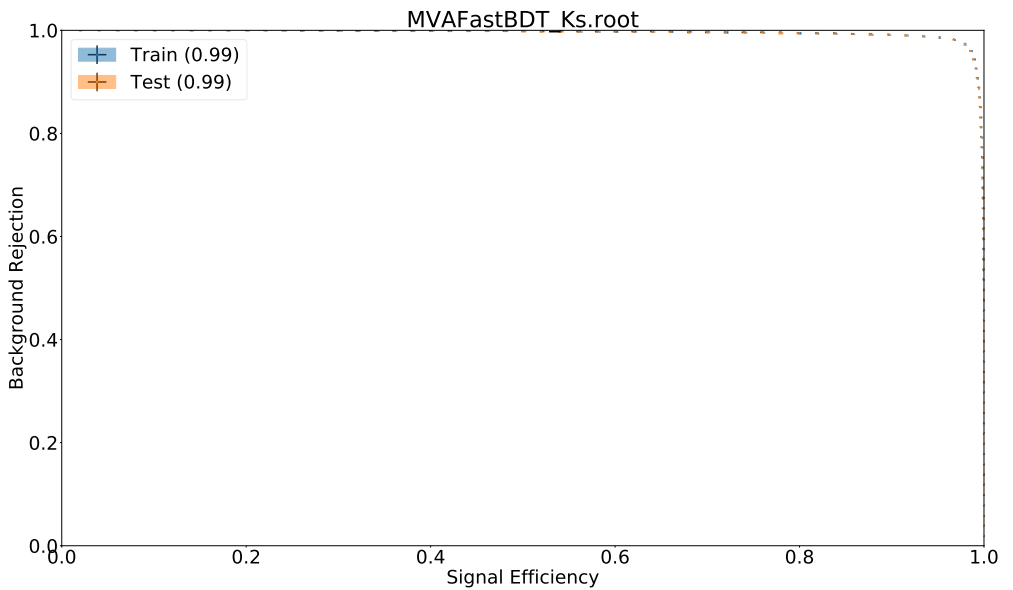
\includegraphics[height=4cm]{jpsi-jpsi}
		\label{fig:side:a}
	\end{minipage}
	\begin{minipage}[b]{0.5\linewidth}
		\centering 
		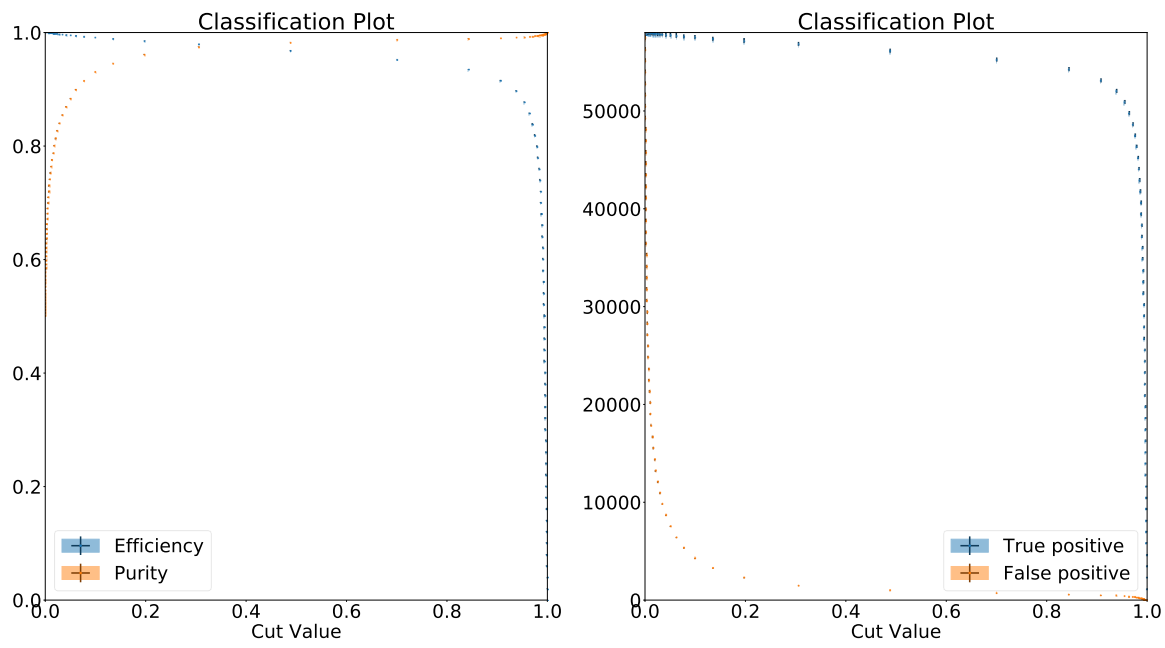
\includegraphics[height=4cm]{jpsi-jpsi-pur}
		\label{fig:side:b}
	\end{minipage}
	\caption{The left is ROC curve and the right is efficiency and purity depending on cut of classifier output. Results are from $B^0 \to J/\psi K_S^0$ generic decay sample.}
\end{figure}
\end{comment}

% 2021.02.08 mid
With increasing the efficiency, the cut on the output of KsFinder is getting loose. The background rejection only starts to drop when the efficiency exceeds about 90\% in both training and testing sample. To be noted, the curves are consistent in training and testing samples. 
While the ROC curve has shown the absence of noticeable over-fitting in classification, the detailed check can be made by comparing the distributions of classifier output on true and fake $K_S^0$ in training and testing samples. Therefore, the distribution of signal and background in training and testing sample with respect to the KsFinder output is plotted, where a distinctive separation for both signal MC and generic MC is shown and no over-training is found, as shown in Figure \ref{fig:ks_overtraining}.
\begin{figure}[H]
	\begin{subfigure}{1\linewidth}
		\centering
		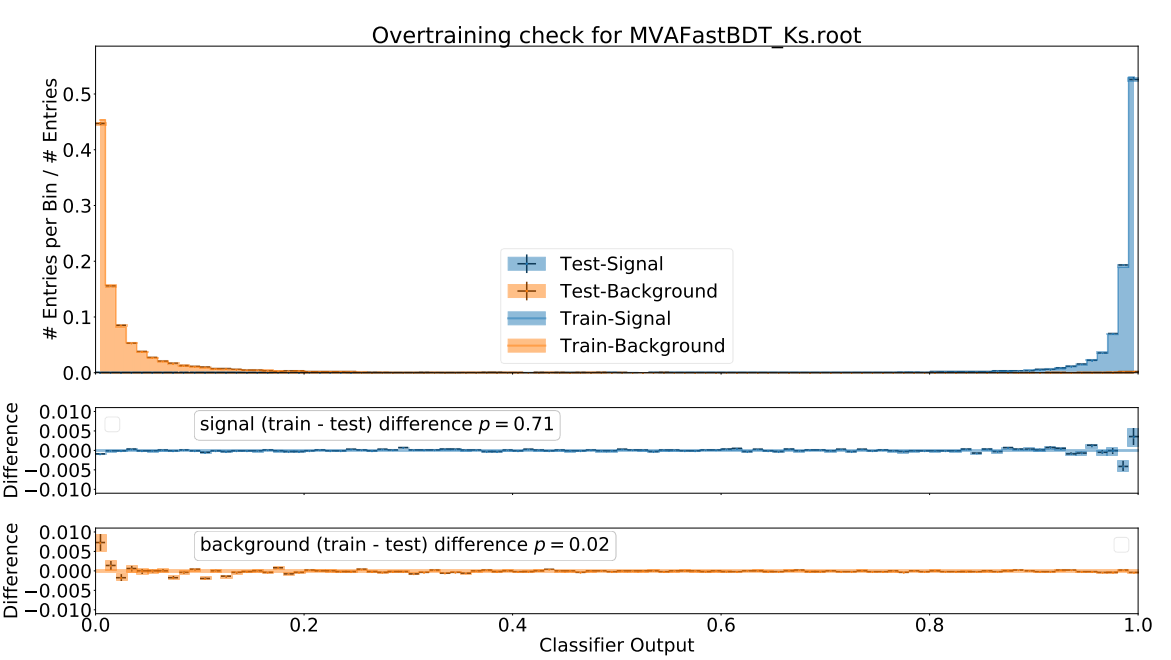
\includegraphics[height=6cm]{over-3ks}
		\caption{Over-fitting check for signal MC sample.}
	\end{subfigure}
  	\vspace{0.3cm}

	\begin{subfigure}{1\linewidth}
		\centering
		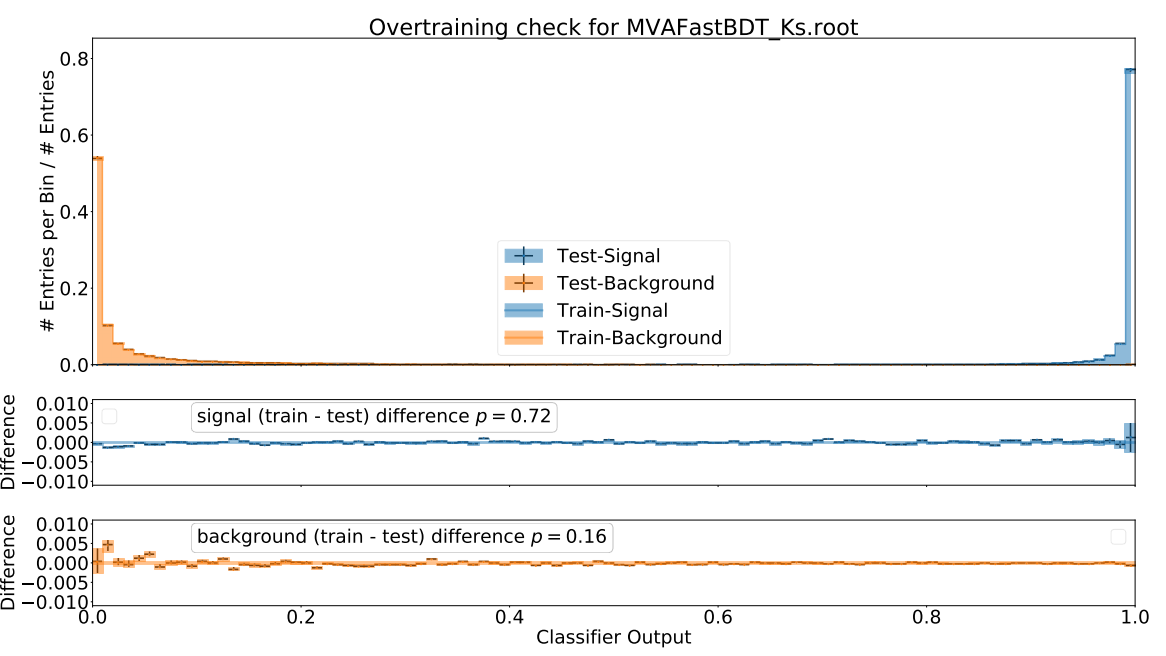
\includegraphics[height=6cm]{over-gen}
		\caption{Over-fitting check for generic MC sample.}
	\end{subfigure}
\caption{The over-training check based on the comparison between training/testing data points in both signal and generic MC.}
\label{fig:ks_overtraining}
	\vspace{0.3cm}
	
%	\begin{subfigure}{1\linewidth}
%		\centering
%		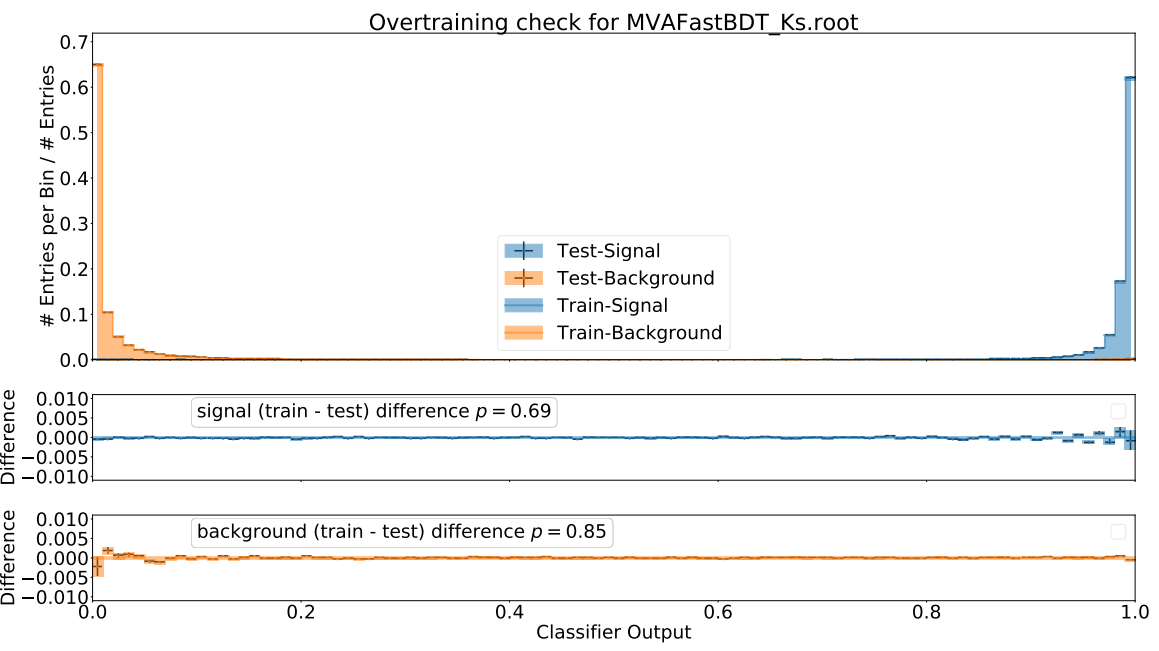
\includegraphics[height=6cm]{over-jpsi}
%		\caption{Over-fitting check for  $B^0 \to J/\psi K_S^0$.}
%	\end{subfigure}
%\caption{Over-fitting check for classifiers.}
\end{figure}

The cut value for \textit{FBDT\_Ks} is determined by maximizing the ``Figure of Merit" (FOM), as shown Equation \ref{eq:fom}, where S and B is the number of true and fake $K_S^0$ after the cut, respectively. The FOM distribution depending on the cut value of FBDT\_Ks is shown in Figure \ref{fig:ks_fom}. The maximum FOM is achieved at FBDT\_Ks $= 0.74$ in signal MC, which is going to be used as the cut value to further reject fake $K_S^0$.

\begin{equation}\label{eq:fom}
	\text{FOM} = \frac{S}{\sqrt{S+B}}
\end{equation}

\begin{figure}[H]
	\centering
	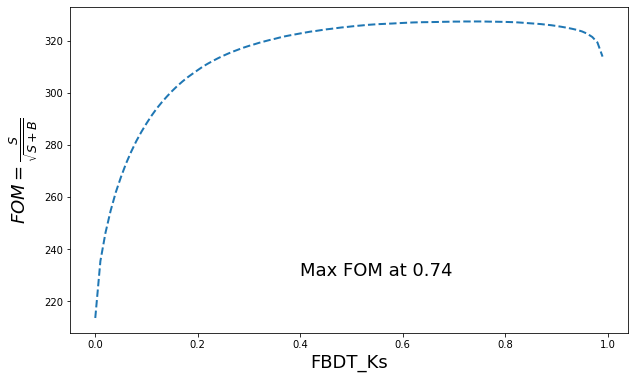
\includegraphics[width=0.6\linewidth]{fom3ks}
	\caption{FOM of classifier output (FBDT\_Ks) in signal MC, the maximum value is achieved at 0.74 and the curve is almost flat between $0.5\sim 0.9$.}
	\label{fig:ks_fom}
\end{figure}

In the signal MC sample, the true $K_S^0$ fraction before applying KsFinder cut is 39\%, and 95.3\% of them are kept after the cut is applied. In the meantime, the fake $K_S^0$ fraction before applying the cut is 61\%, and 97.6\% of them are rejected after the cut is applied. The purity of the $K_S^0$ candidates is improved largely as shown in Figure \ref{fig:ks_cutused}.

\begin{figure}[htpb]
	\centering
	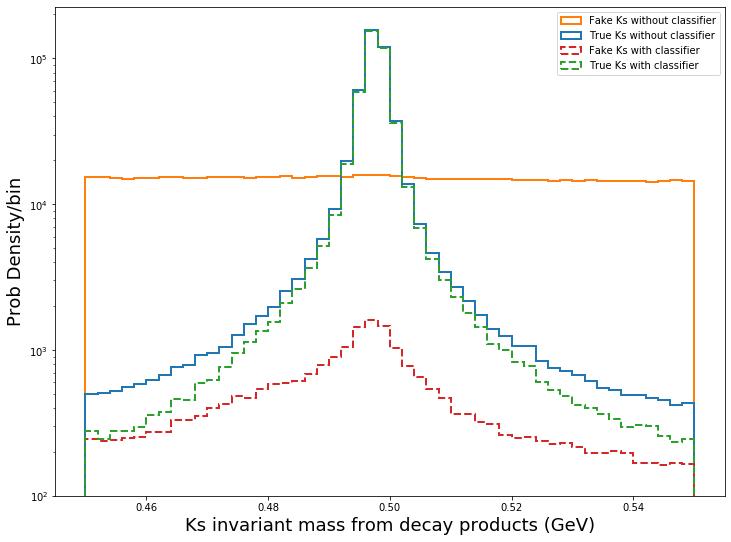
\includegraphics[width=0.7\linewidth]{kscutM}
	\caption{$K_S^0$ purity improvement with cut value of FBDT\_Ks at 0.74 applied. The blue solid line is true $K_S^0$ without KsFinder and green dashed line is the true $K_S^0$ with the cut applied. The orange solid line is fake $K_S^0$ without the cut and the red dashed line is fake $K_S^0$ with the cut. About 95.3\% of true $K_S^0$ are kept while 97.6\% of the fake ones are rejected by applying the cut.}
	\label{fig:ks_cutused}
\end{figure}

%2021/02/17 mids
\subsection{Data Validation for Classifier}
The results from MC studies show an excellent performance of KsFinder. However, the validation of such a tool on the real experiment data is necessary. Since there's no MC truth on target variable in real data, the FastBDT method is based on variables in MC samples. If these variables shows close distribution among MC and data, the classification performance is expected to be similar.

In addtion, due to the fact that $K_S^0$ candidates are used for further reconstruction of $B^0$, the  mass and energy distributions may change after applying the cut, thus the validation that approves no clear bias on $B^0$'s variables that are used for signal extraction is also required. For comparison between MC and data, a small data sample from Belle II  experiment 7 and 8 is used. The integral luminosity at $\Upsilon(4S)$ resonance for this data sample is about 5.17 $\text{fb}^{-1}$. The MC sample is extracted from generic MC with equivalent events number which includes two types of MC: \textit{MC12b} is the one produced in early 2019, and the latest MC in 2020.

%0217 ends

 The Figure \ref{fig:ksvalid_1} shows the invariant mass and momentum distributions from data and MC samples, and full comparison of all training variables is included in Appendix B. 
 
 It shows that kinematics of $K_S^0$ in data and MC yield fairly close distributions and no clear bias is seen by applying the KsFinder cut.

\begin{figure}[H]
	\begin{subfigure}{0.5\linewidth}
		\includegraphics[page=2,height=4cm]{dataVarsPlot_Ks.pdf}
	\end{subfigure}
	\begin{subfigure}{0.5\linewidth}
		\includegraphics[page=7,height=4cm]{dataVarsPlot_Ks.pdf}
	\end{subfigure}
	\bigskip
	\begin{subfigure}{0.5\linewidth}
		\includegraphics[page=8,height=4cm]{dataVarsPlot_Ks.pdf}
	\end{subfigure}
	\begin{subfigure}{0.5\linewidth}
		\includegraphics[page=9,height=4cm]{dataVarsPlot_Ks.pdf}
	\end{subfigure}
\caption{The distribution of invariant mass from charged pions and the momentum of $K_S^0$ in $x,y,z$ directions. Blue bar is from all MC13, cyan bar is the true $K_S^0$ in it. Yellow step histogram is data with no cut, solid red data with MC13 trained cut, and the dashed is with MC12b cut. Experimental data has a good agreement with MC before and after applying the KsFinder.}
\label{fig:ksvalid_1}
\end{figure}

\subsection{KsFinder Effects on Kinematics Evaluation}
Implementing KsFinder for $K_S^0$ may induce extra bias on the event numbers for $K_S^0$. It's not easy to direct evaluate the impact of each variables in training towards the final signal yield because the output is non-linear dependence on those variables. However, we can directly use the output of KsFinder and introduce the scale factor when check the data and MC signal yields. 
 
A fit on invariant mass $M$ of $K_S^0$ candidates after varied cut on KsFinder output is done by modeling signal shape as double-Gaussian and background as Chebyshev polynomial. Significance is define as $S_{data/MC} = N_{signal} /N_total$ in data and MC from fitting using RooFit. A list of intervals of cut value on KsFinder output is made and the significance is calculated within each interval. Fitting results are shown in Fig 3.17 using loose and tight cut respectively. The fit plots in all cut intervals are included in Appendix C.  Data/MC correction is defined as:

\begin{equation}
	R = \frac{S_{MC}}{S_{data}}
\end{equation}



\begin{figure}[htpb]
	\begin{subfigure}{0.5\linewidth}
		\caption{Data,cut=0.2}
		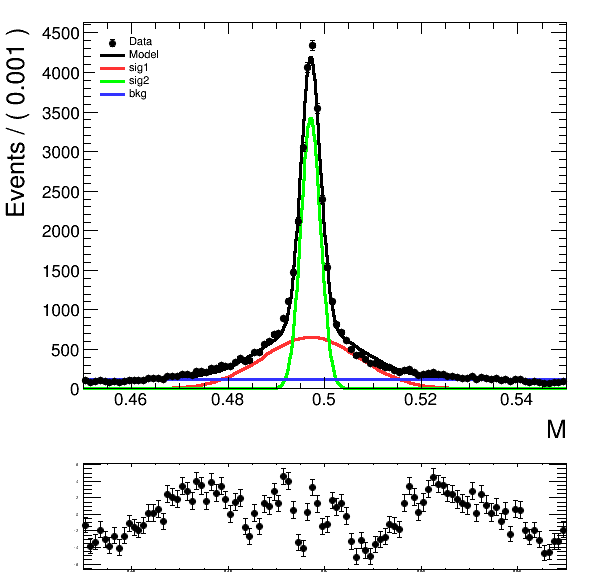
\includegraphics[width=1\linewidth]{ksDatamva0.2.png}
	\end{subfigure}
\begin{subfigure}{0.5\linewidth}
	\caption{MC,cut=0.2}
	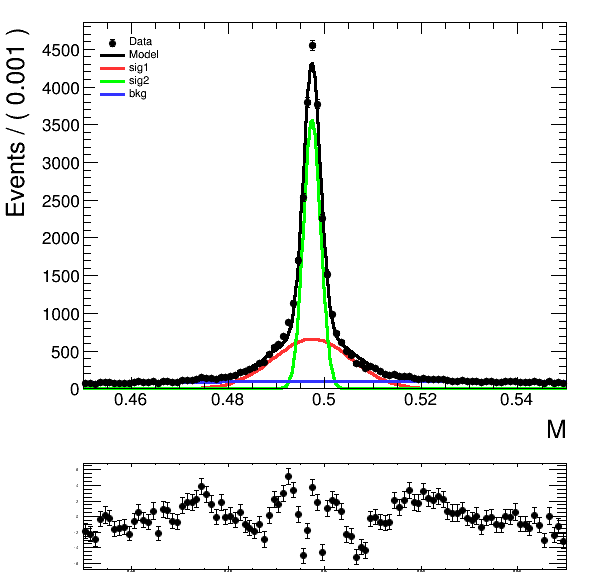
\includegraphics[width=1\linewidth]{ksMCmva0.2.png}
\end{subfigure}

\begin{subfigure}{0.5\linewidth}
	\caption{Data,cut=0.9}
	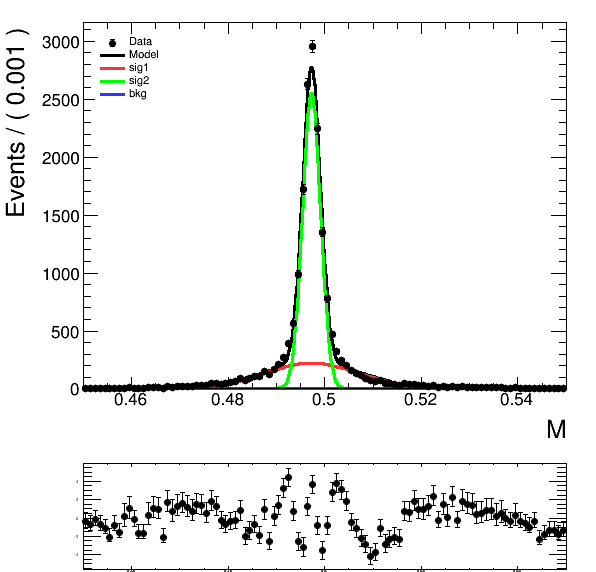
\includegraphics[width=1\linewidth]{ksDatamva0.9.png}
\end{subfigure}
\begin{subfigure}{0.5\linewidth}
	\caption{MC,cut=0.9}
	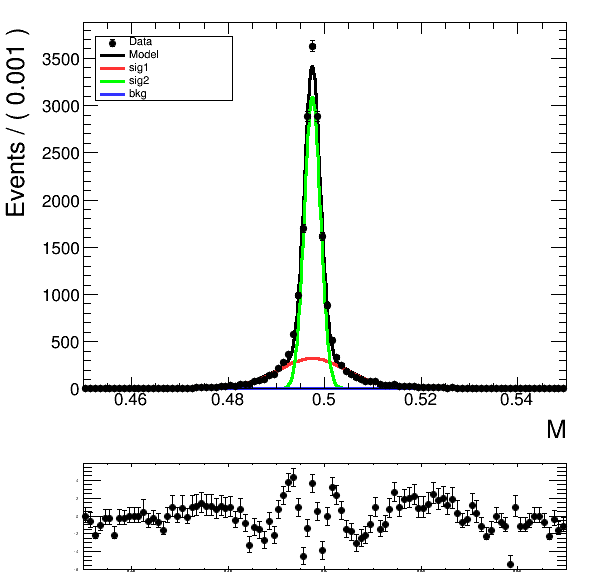
\includegraphics[width=1\linewidth]{ksMCmva0.9.png}
\end{subfigure}
\caption{Invariant mass fit of $K_S^0$ using cut at 0.2(loose) and 0.9(tight) to calculate $S_{data/MC}$.}
\end{figure}

The correction is defined by taking the R value within the chosen interval. Uncertainty of R is defined by the difference of maximum and minimum of R in all intervals. R is distributed as: 
\begin{figure}[H]
	\centering 
	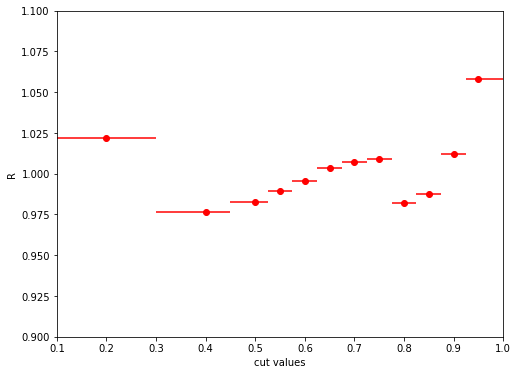
\includegraphics[width=0.7\linewidth]{Rc}
	\caption{Data MC correction induced by $K_S^0$ classifier.}
\end{figure}

The R, for example in cut value 0.74 of maximum FOM, is $R = 1.009\pm 0.081$. In $B^0 \to K_S^0  K_S^0  K_S^0$, the correction of $B^0$ events should be proportional to R to the three.  Correction that is implemented for $B^0$ is $1.027^{+0.33}_{-0.18}$. In most of the cut intervals, the R is within 2.5\% so the bias on $K_S^0$ numbers is very small.
\begin{comment}
\subsection{Summary}
The development of Belle II $K_S^0$ classifier is enlighten by the experience from Belle. A comprehensive study of training observables from $K_S^0$ decay characteristics has been exploited. It takes the advantage of FastBDT algorithm to achieve a high fake rejection power. As a result, classifier is able to give a output which can be used as a cut to select good $K_S^0$ candidates with high purity. The classifier is validated with real experimental data as well. A primary data validation study of KsFinder is conducted with implementing correction on data and MC along with its contribution to $B^0$. The performance of KsFinder is in a good shape and no clear bias is found on the yield of the number of $K_S^0$. For the reconstruction of $B^0 \to K_S^0  K_S^0  K_S^0$, the development of KsFinder is critical to suppress large fraction of combination background from fake $K_S^0$.
\end{comment}
